\documentclass[9pt,twocolumn,twoside,lineno]{gsajnl}
% Use the documentclass option 'lineno' to view line numbers

%\articletype{inv} % article type
% {inv} Investigation 
% {gs} Genomic Selection
% {goi} Genetics of Immunity 
% {gos} Genetics of Sex 
% {mp} Multiparental Populations

\title{The Genetics of Phospholipid Metabolism In Maize Highland Adaptation}

\author[$\ast$,$\dagger$, 1]{Fausto Rodríguez-Zapata}
\author[$\dagger$, 1]{Karla Blöcher-Juárez}
\author[$\dagger$]{Rocío Aguilar-Rangel}
\author[$\dagger$]{Juan M Estévez-Palmas}
\author[$\ddagger$]{Dan Gates}
\author[$\S$]{Garret Janzen}
\author[$\dagger$]{Sergio Pérez-Limón}
\author[$\S$]{Li Wang}
\author[$\ast\ast$]{Oliver Fiehn}
\author[$\S$]{Matthew Hufford}
\author[$\ddagger$]{Jeffrey Ross-Ibarra}
\author[$\dagger$,$\dagger\dagger$]{Ruairidh JH Sawers}
\author[$\ast$,$\dagger$, 2]{Rubén Rellán-Álvarez}

\affil[$\ast$]{Department of Molecular and Structural Biochemistry, North Carolina State University, Raleigh, NC}
\affil[$\dagger$]{National Laboratory of Genomics for Biodiversity, Irapuato, México}
\affil[$\ddagger$]{Department of Ecology, Evolution, and Organismal Biology, Iowa State University, Ames, USA}
\affil[$\S$]{Department of Evolution and Ecology, Center for Population Biology and Genome Center, University of California, Davis, CA}
\affil[$\ast\ast$]{West Coast Metabolomics Center, University of California, Davis, CA, USA}
\affil[$\dagger\dagger$]{Department of Plant Science, The Pennsylvania State University, PA, USA}

\keywords{phospholipid metabolism; maize genetics; highland adaptation; convergent evolution}

\runningtitle{Phospholipid Pathway Selection in Highland Maize} % For use in the footer 

%% For the footnote.
%% Give the last name of the first author if only one author;
% \runningauthor{FirstAuthorLastname}
%% last names of both authors if there are two authors;
% \runningauthor{FirstAuthorLastname and SecondAuthorLastname}
%% last name of the first author followed by et al, if more than two authors.
\runningauthor{Rodríguez-Zapata, Blöcher-Juárez \textit{et al.}}

\begin{abstract}
After domestication from lowland teosinte in the warm, humid Mexican southwest maize colonized the highlands of Mexico and South America. In the highlands, maize was exposed to a whole range of environmental factors that differ from the site of domestication, including, among others, lower temperatures, soils with lower phosphorus availability and different biological pressures. In my talk, I will present data supporting the hypothesis that glycerolipid metabolism remodeling was important in the process of maize adaptation to highlands. I will show results from common garden experiments in Mexican lowland and highland common gardens where we grew maize mapping populations and using quantitative biochemical genetics tools we identified major QTLs that explain the conversion of phosphatidylcholines (PCs) to lyso-phosphatidylcholines (LPCs) leading to a high PC/LPC ratio that is particularly conserved in Mexican highland landraces. Using GBS data from 4000 maize landraces and whole genome sequences from another 30 landraces across the Americas we found that candidate genes underlying this QTL and others coding for PCs to/from LPCs conversions also show clear signs of selection to highlands. I will present ongoing work to identify the causative SNPs on candidate genes that lead to this biochemical phenotype, their natural variation and ultimately the physiological mechanisms that are affected by it and their role in maize highland adaptation. 
\end{abstract}

\begin{document}

\maketitle
\thispagestyle{firststyle}
%\marginmark
\firstpagefootnote
\equalcontrib{1}
%\equalcontrib{2}

\correspondingauthoraffiliation{3}{Department of Molecular and Structural Biochemistry, North Carolina State University, 27607, Raleigh, NC. Email: rrellan@ncsu.edu}
\vspace{-33pt}% Only used for adjusting extra space in the left column of the first page

\lettrine[lines=2]{\color{gray}M}aize (\textit{Zea mays spp. mays}) was domesticated in the tropical basin of the Balsas River (Guerrero, Mexico) around 10,000 years ago from the wild relative teosinte parviglumis (\textit{Zea mays spp. parviglumis}) \citep{Matsuoka2002-bg,Piperno2009-fj}). 
After domestication, maize expanded throughout México, north into the US \citep{Da_Fonseca2015-zh} and south into Central America and South America (Wang et al., 2017) and has been adapted to a wide diversity of environments and today is grown in a wider geographical range than any other crop \citep{Hake2015-or}.  
Maize has also adapted to a wide variety of uses, from the myriad culinary applications of local communities growing maize landraces particularly in Mexico \citep{Bellon2018-cm} to the diverse range of products (from ethanol to high fructose syrup) that are produced with modern hybrids in modern agronomical operations. 
The genetic changes that lead to maize domestication \citep{Doebley1995-su,Doebley1997-oy, Wang2005-by, Clark2006-xh,Dorweiler1993-ik} and maize adaptation to a wider latitudinal range \citep{Liang2018-af, Guo2018-on, Coles2010-db, Huang2018-ga, Yang2013-lg, Salvi2007-ku, Wang2017-oz} provide a relatively good understanding of the genetic regions and mechanism that shaped maize domestication and latitudinal expansion. 
However, the mechanisms involved in maize landrace local adaptation that enabled maize to adapt to such a diverse range of environmental conditions are still largely unknown. 

In this paper, we posit  phospholipid pathways are under selection in highland balance had an important role in maize adaptation to highlands.  
Our hypothesis is based on what we know about how plants respond to a number of environmental conditions that are characteristic of highlands and that affect phospholipid metabolism and conferred an adaptive significance as maize colonized highland territory. 
Phospholipid concentration increase \citep{Degenkolbe2012-wf} together with a reduction of glycerolipids with highly saturated fatty acids \citep{Welti2002-uk}(Welti et al., 2002) are two of the strategies plants use to respond to cold temperatures \cite{Lynch1987-ln}. 
These changes are supposed to help maintain the fluidity of plasma membranes at colder temperatures. On the other hand, plants adapted to low phosphorus conditions degrade phospholipids and increase the concentration of glycerolipids and sulpholipids (Lambers et al., 2012), particularly, in older leaves to free up phosphorus. 
The highlands of Mexico, and particularly the Trans-Mexican volcanic belt are characterized volcanic soils with low phosphorus availability (Krasilnikov, P., Gutiérrez-Castorena, M.d.C., Ahrens, R.J., Cruz-Gaistardo, C.O., Sedov, S., Solleiro-Rebolledo, E, 2013). 
In the regions where maize is grown in Mexico, there is a positive correlation between altitude and phosphorus retention (Zapata, 2018). 
As maize adapted to higher elevations with lower phosphorus availability and colder temperatures, phospholipid metabolism faced contrasting selective pressures. 
Cold temperatures also affect maize development. Farmers can predict flowering dates using Growth Degree Units (GDU) that takes into account the maximum and minimum temperatures on a given day. 
Maize needs between 800 and 1400 GDU to reach maturity. 
In Mexican highland conditions, growing degree days are usually around 5 GDU while in lowlands they are 15 GDU. 
It takes a maize plant around 3 times longer to reach maturity in highland than in lowland conditions. To deal with these lower GDUs, highland maize landraces are planted early in the season (February-March) and harvested around November. 
In maize, glycerolipid content has a high flowering time predictive power (Riedelsheimer et al., 2013). 
The high predictive predictive power of flowering time by glycerolipids could be explained at the molecular level by the discovery that certain phosphatidylcholine species bind to flowering locus T and accelerate flowering time through a yet unknown mechanism (Nakamura et al., 2014). 
Highland adapted landraces have short flowering times probably as an adaptive strategy to deal with low GDU values in the highlands.   
Several lines of evidence indicate that glycerolipid metabolism was under selection in independent events of maize highland adaptation. 
Takuno and collaborators used Fst statistics to identify loci that were under selection in both Mesoamerica and South America highland maize (Takuno et al., 2015). 
They found little evidence of convergence between the two sub continents but glycerolipid pathways were under the few pathways that showed convergence at the pathway level (Takuno et al., 2015). 
We have also found that Palomero Toluqueño (a Mexican highland landrace) has higher concentrations than B73 of the same phosphatidylcholine species that bind to FT and accelerates flowering (Nakamura et al., 2014).
In this paper we set out to study the possible role glycerolipid and in particular phospholipid metabolism in the process of maize adaptation to highland conditions. 
Using a multi pronged approach that combined QTL analyses of phospholipid content biparental RIL mapping made of a cross of B73 and Palomero Toluqueño (a highland landrace), phospholipid analysis in a 120 landrace diversity panel, analysis of genome wide signals of selection to highland altitude using WGS of 30 landraces and GBS data of 2700 landraces we identified candidate loci at that were both under selection in highland maize and that show phospholipid quantitative variation  in biparental populations. 
In particular, our analysis identified a major QTL controlling phosphatidylcholine and lyso-phosphatidylcholine levels. A phospholipase type A1 (\textit{ZmPLa1.2}) that shows strong signals of selection in highland maize and is located at the peak of the QTL. Further analysis using the genetic materials generated in this paper will allow us to test the adaptive significance of this metabolic trait to maize adaptation to highland conditions and will help to better understand if natural variation in the candidate loci could be used to improve modern maize varieties that face similar environmental conditions than highland maize like early season cold stress. 

\section{Materials and Methods}
\label{sec:materials:methods}

\subsection{Populations used in the analysis } 
B73 x PT RILs
Hilo Panel
Li genomes (can cite Li 2017)

We used landraces individual accessions genotypic data from the CIMMYT Seeds of Discovery project (SeeD). The SeeD project has genotyped 24,000 landraces from the  CIMMYT International Germplasm Bank maize collection primarily from American origin.


\subsection{Field Experimental Conditions} 
Here we also include some comparisons between the greenhouse plants and plants of the same genotype grown in a highland field. In the field, 8 plants per genotype were sampled, in a field located in Metepec, Mexico State, (19°13'28.7"N 99°32'51.6"W) within the Trans-Mexican volcanic belt. The field is placed at 2610 meters above sea level (masl), the range of average monthly temperatures along the year vary from 5 °C to 21.5 °C with an average annual of 13.6 °C. The field samples were collected between 10:00 am and 12:00 pm, approximately 3 h after sunrise.  From all plants 50 mg of fresh tissue was collected from the tip of the S2 leaf (two leaves younger of the last leaf with a fully developed collar), when the plants were around the V5 developmental stage. 

\subsection{Lipid extraction and UHPLC-QTOF MS/MS lipid profiling} 

We collected fifty mg of leaf tissue using a leaf puncher and fast froze it in liquid nitrogen. Frozen material was homogenized in a tissue grinder Retsch (Haan, Germany) for 40 seconds at a frequency of 30 1/s. After grinding, samples were extracted. 
We performed lipid extraction as reported by Matyash and collaborators (Matyash et al. 2008). 
First, 225 $\mu$L of cold methanol (MeOH), was added to each sample. 
For the blanks, MeOH previously prepared with a Quality Control (QC) mix was added (Supplementary Table XX). Each sample was vortexed for 10 seconds, keeping the rest of materials on ice. 
Then 750 $\mu$L of cold methyl tert-butyl ether (MTBE) were added. The MTBE added to the blanks contained 22:1 cholesterol ester as internal standard (Supplementary Table XX). 
Each sample was vortexed for 10 seconds, followed by 6 minutes of shaking at 4°C in the orbital mixer. 
188 $\mu$L of LC/MS grade water at room temperature (RT) was added, and the samples were vortexed for 20 seconds.
We centrifuged the samples for 2 min at 14000 rcf (12300 rpm) and recovered 700 $\mu$L of supernatant from the upper organic phase. 
We then split the supernatant two aliquots of 350 $\mu$L, one for lipid profiling and the other for preparation of pools to be used along the lipid profiling. 
Finally, samples were dried with a speed vacuum concentration system.
Dry samples were resuspended in 110 $\mu$L of MeOH-Toluene 90:10 (with the internal standard CUDA, 50 ng/mL). 
Samples were vortexed at low speed for 20 s and then sonicated at RT for 5 min. 
Aliquots of 50 $\mu$L per sample were transferred into an insert within an amber glass vial.
The UHPLC-QTOF MS/MS utilized were Agilent 1290 and Agilent 6530, respectively. 
Before analyzing the samples a new Waters Acquity charged surface hybrid (CSH) C18 2.1x100 mm 1.7 $\mu$m column was set. 
The column was initially purged for 5 min. 
The UHPLC column was coupled to a VanGuard pre-column (Waters Acquity CSH C18 1.7$\mu$m). 
Six “no sample injections” were injected at the beginning of each run to condition the column, followed by ten samples, one pool (made out of the mix of the second aliquot of all the samples contained per UHPLC plate) and one blank.
We injected 1.67 $\mu$L per sample into UHPLC-QTOF MS/MS ESI (+), the running time per sample was 15 min. Mobile phase “A” consisted of 60:40 acetonitrile:water, 10 mM of ammonium formate and 0.1\% formic acid. 
Mobile phase “B” consisted of 90:10 isopropanol:acetonitrile, 10 mM ammonium formate and 0.1\% of formic acid. 
The flow rate was maintained at 0.6 mL/min and the column compartment was maintained at 65 °C. Initial conditions were 15\% B; the gradient uniformly increased until reaching 100\%. 
At 12.10 min the mobile phase composition returned to initial conditions.

The mass spectrometer (QTOF MS/MS) was operated in positive electrospray ionization mode (ESI), based on the diversity and amount of lipid species identified under ESI (+) and (-) during the lipid profiling optimization (See supplementary Table 3) on Agilent® ultra high performance liquid chromatography and quadrupole time of flight mass spectrometry (UHPLC-QTOF MS). For this optimization we used 8 samples of B73, 8 samples of PT and 10 samples of a recombinant inbred line population (RILs) generated by crossing B73 and PT, only MS1 data was acquired. Same samples were utilized for both ESI modes. 
Under positive mode 24 lipids were identified, having two cholesterol esters (CE), 3 diacylglycerols (DG), 2 lysophosphatidylcholines (LPC), 10 phosphatidylcholines (PC), 1 phosphoethanolamine (PE) and 6 triacylglycerols (TG). 
While under negative mode we identified 16 lipids, of which, 14 were fatty acids (FA) and 2 were PC species. 
For the source parameters, ESI gas temperature was set at 325 °C, nebulizer pressure of 35 psig, gas flow of 11L/min, capillary voltage at 3500 V, nozzle voltage at 1000V, MS TOF fragmentor and skimmer at 120 and 65 V, respectively. 
Under the acquisition parameters a mass range between 60 and 1700 m/z was set. As for reference mass parameters, a detection window of 100 ppm and a minimum height of 1000 counts were set. 

\subsection{Data Availability}

At the end of the Materials and Methods section, include a statement on reagent and data availability. Please read the Data and Reagent Policy before writing the statement. Make sure to list the accession numbers or DOIs of any data you have placed in public repositories. List the file names and descriptions of any data you will upload as supplemental information. The statement should also include any applicable IRB numbers. You may include specifications for how to properly acknowledge or cite the data.

For example: Strains are available upon request. File S1 contains detailed descriptions of all supplemental files. File S2 contains SNP ID numbers and locations. File S3 contains genotypes for each individual. Sequence data are available at GenBank and the accession numbers are listed in File S3. Gene expression data are available at GEO with the accession number: GDS1234. Code used to generate the simulated data is provided in file S4. 


\section{Results}
\label{sec:results}

\subsection{Glycerophospholipid pathways are under selection in  highland maize} 
We analyzed selection of glycerolipid related pathways in highland maize using several approaches. 
We first selected 211 genes that are in glycerolipid related enzymatic pathways from the Plant Metabolic Network (Schläpfer et al., 2017). 
We then used the Population Branch excess (PBE) statistic (Pool et al., 2017), to analyze if glycerolipid pathway genes are under selection in highland populations. 
PBE quantifies changes in allele frequencies in focal populations relative to two independent “outgroup” populations. 

\begin{figure*}[!ht]
\begin{center}
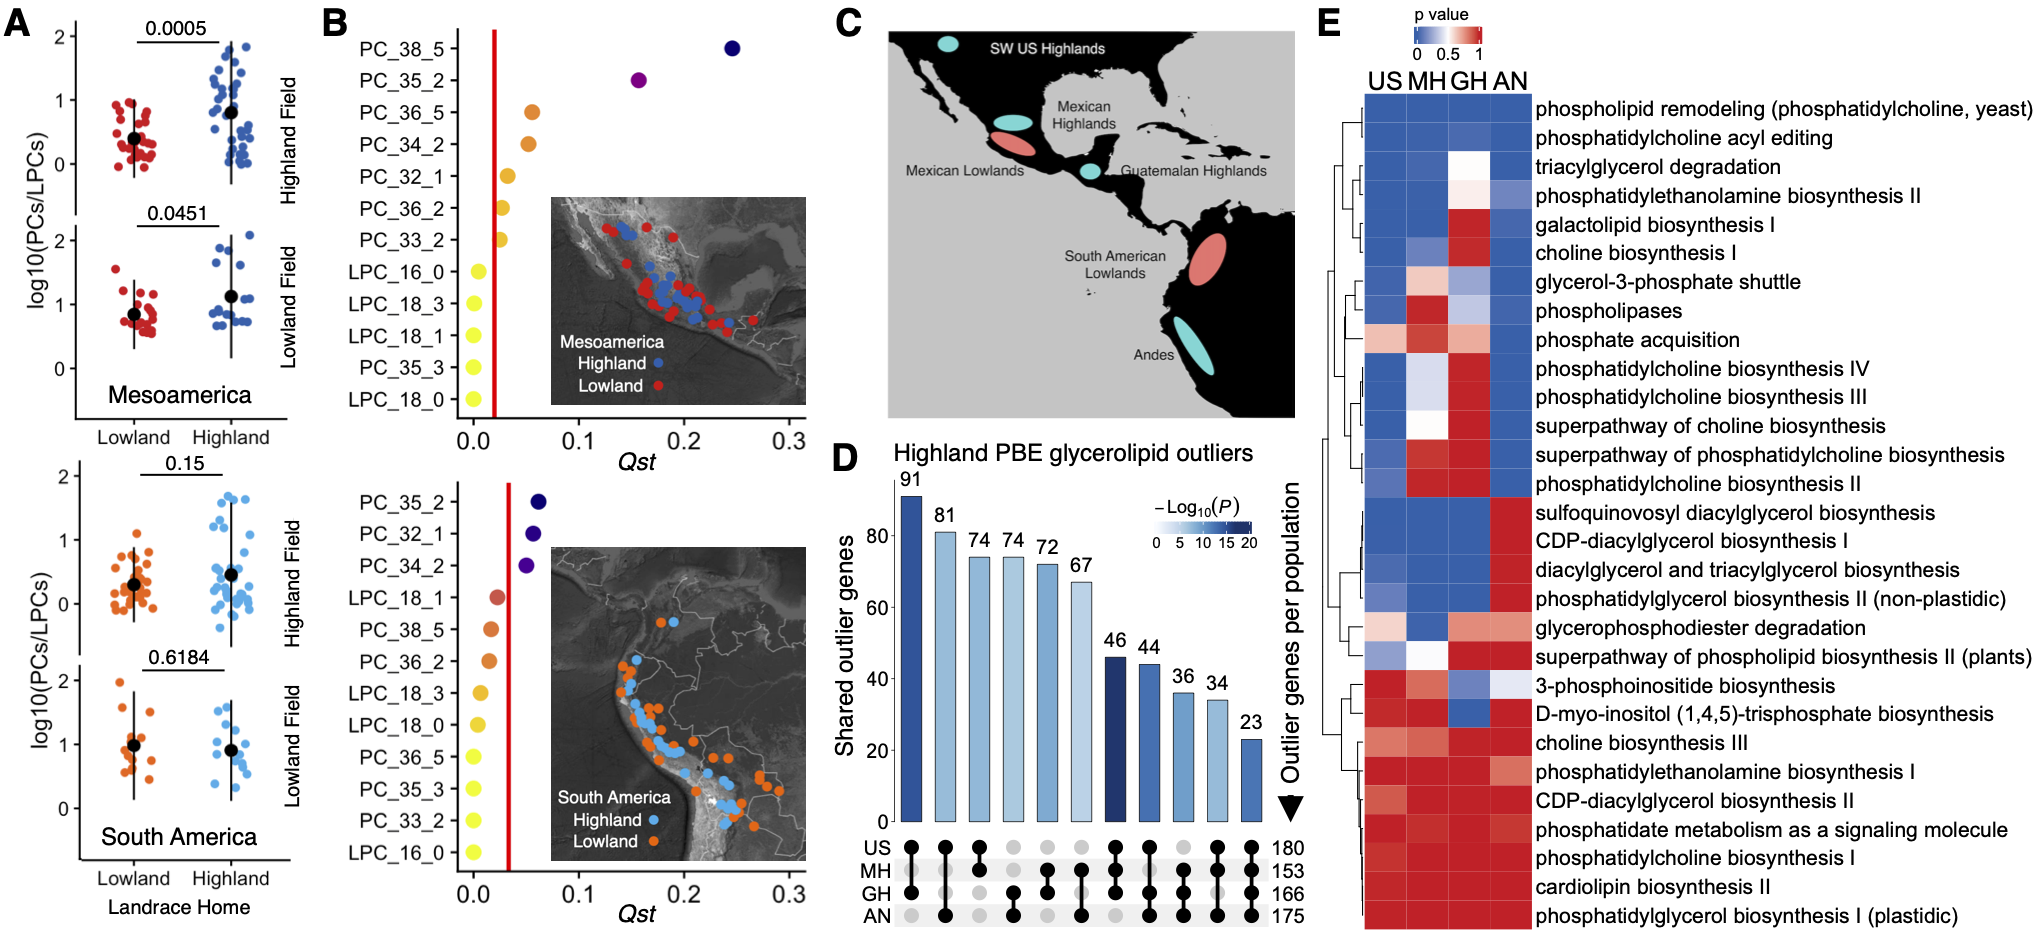
\includegraphics[width=0.8\paperwidth]{Figures/Fig_1.png}
\caption{Glycerolipid pathway selection 
A) Populations used in the Population Branch Excess (PBE)analysis. 
B) Mean PBE values of SNPs located within 10Kb flanking glycerolipid enzyme genes for each highland population are show in red lines against the genomic background distribution. 
C) Intersection of glycerolipid pathways related genes among the four highland populations. 
D) Map showing the geographical origin of the 120 accessions used in the common garden experiment to quantify glycerolipid compounds. 
E) Correlation between  lyso-phosphatydilcholine (LPC) species and the ratio of  phosphatydilcholine (PCs) species and LPC species. 
F) Logaritmic values of the PC/LPC ratio of highland and lowland landraces from Mesoamerica.}
\label{PBE_Qst-Fst}
\end{center}
\end{figure*} 

We performed PBE analysis in four different highland populations: Southwest US, Mexican Highlands, Guatemalan Highlands and Andes and used a Mexican Lowland population -in the case of Southwest US, Mexican and Guatemalan Highlands- or a South American Lowland -in the case of Andes- (Fig 1A) (Wang et al., 2017) and teosinte parviglumis (Zea mays spp. parviglumis) as the two outgroups. 
When compared with a random sampling distribution of PBE values, the median PBE value of glycerolipid pathway genes was significantly higher indicating that glycerolipid pathway genes are under selection in all 4 highland populations (Fig 1B). 
Twenty three genes were under selection in at least three highland populations (Fig 1C, table 1 and Supplementary Table 1) and the majority of them are genes involved in the synthesis and degradation of phospholipids. 
Among these we find several types of phospholipases (Ryu, 2004) such as Zm00001d039542 (PLA1 type) Zm00001d029955 (PLA2 type), Zm00001d014386 (PLAT-PLA type) and lyso-phospholipd acylases such as Zm00001d017584 and Zm00001d007638 (ZmPls1).  
These two types of genes are involved in determining the relative abundance of phospholipids and lyso-phospholipids. 

%\begin{table*}[htbp]
% \caption{\bf PBE outlier genes in at least 3 highland populations and \textit{pcadapt} -logP values}
% \begin{tableminipage}{\textwidth}
% \begin{tabularx}{\textwidth}{XXXX}
% \hline
% Gene ID        & US & MH & GH & AN & Sum & Function       & \_-logP pcadapt \\
% Zm00001d048835 & 1  & 1  & 1  & 1  & 4   & PL degradation & 39.2            \\
% Zm00001d014386 & 1  & 1  & 1  & 1  & 4   & PL degradation & 6.9             \\
% Zm00001d017584 & 1  & 1  & 1  & 1  & 4   & PL synthesis   & 99.3            \\
% Zm00001d045927 & 1  & 1  & 1  & 1  & 4   & DG degradation & 40.1            \\
% Zm00001d018593 & 1  & 1  & 1  & 1  & 4   & DG synthesis   & 31.9            \\
% Zm00001d018595 & 1  & 1  & 1  & 1  & 4   & SL Synthesis   & 31.9            \\
% Zm00001d029955 & 1  & 1  & 1  & 0  & 3   & PL degradation & 1.1             \\
% Zm00001d033683 & 0  & 1  & 1  & 1  & 3   & PL degradation & 1.4             \\
% Zm00001d039542 & 1  & 1  & 1  & 0  & 3   & PL degradation & 110.3           \\
% Zm00001d013935 & 1  & 1  & 1  & 0  & 3   & PL synthesis   & 0.8             \\
% Zm00001d007638 & 1  & 1  & 1  & 0  & 3   & PL synthesis   & 0.0             \\
% Zm00001d020647 & 1  & 1  & 1  & 0  & 3   & PL synthesis   & 24.0            \\
% Zm00001d018594 & 1  & 1  & 1  & 0  & 3   & DG synthesis   & 31.9            \\
% Zm00001d053009 & 1  & 1  & 1  & 0  & 3   & TG Synthesis   & 1.5             \\
% Zm00001d039274 & 1  & 1  & 1  & 0  & 3   & TG Synthesis   & 5.0             \\
% Zm00001d028482 & 1  & 0  & 1  & 1  & 3   & PL degradation & 15.3            \\
% Zm00001d004913 & 1  & 0  & 1  & 1  & 3   & PL degradation & 0.9             \\
% Zm00001d044052 & 1  & 0  & 1  & 1  & 3   & PL degradation & 16.7            \\
% Zm00001d005770 & 1  & 0  & 1  & 1  & 3   & PL degradation & 0.7             \\
% Zm00001d006507 & 1  & 0  & 1  & 1  & 3   & PL degradation & 23.6            \\
% Zm00001d032973 & 1  & 0  & 1  & 1  & 3   & PL synthesis   & 30.7            \\
% Zm00001d028698 & 1  & 0  & 1  & 1  & 3   & PL synthesis   & 8.3             \\
% Zm00001d048766 & 1  & 0  & 1  & 1  & 3   & PL synthesis   & 1.8            
% \hline
% \end{tabularx}
%   \label{tab:shape-functions}
% \end{tableminipage}
% \end{table*}

These results indicate that glycerolipid pathway genes and in particular genes involved in phospholipid metabolism are under convergent selection in all four highland populations. 
We then analyzed if the levels of phospholipids varied between highland and lowland landraces. 
We grew a panel of 120 landraces selected from highland (> 2000 masl) and lowland (<1000 masl) from Mesoamerica and South America (Fig 1D, Supplementary Table 2) in a common garden experiment in Metepec, Edo de México.
This field is located at 2600 masl and represents a typical highland environment of central Mexico. 
We sampled plants at V4-V6 developmental stages and we analyzed glycerolipid composition using LC-MS. We analyzed the levels phosphatidylcholine (PC) and lyso-phosphatydilcholine (LPC) species, the most abundant phospho/lyso-phospholipid species. 
We found that the ratios of the sums of PCs over LPcs species were significantly higher in highland landraces than in lowland landraces, particularly in landraces from Mesoamerica.  
This high ratio is driven by low levels of lyso phosphatydilcholine species (Fig 1E-F, Supplementary Fig 1).

We also genotyped the individual plants that were used for glycerolipid analysis and conducted Qst-Fst analysis on the landraces glycerolipid data. 
The majority of glycerolipid species we quantified showed Qst values higher than Fst when we compared between highland and lowland populations from Mesoamerica and South America (Supplementary Fig 2). 

\begin{figure}[!ht]
\begin{center}
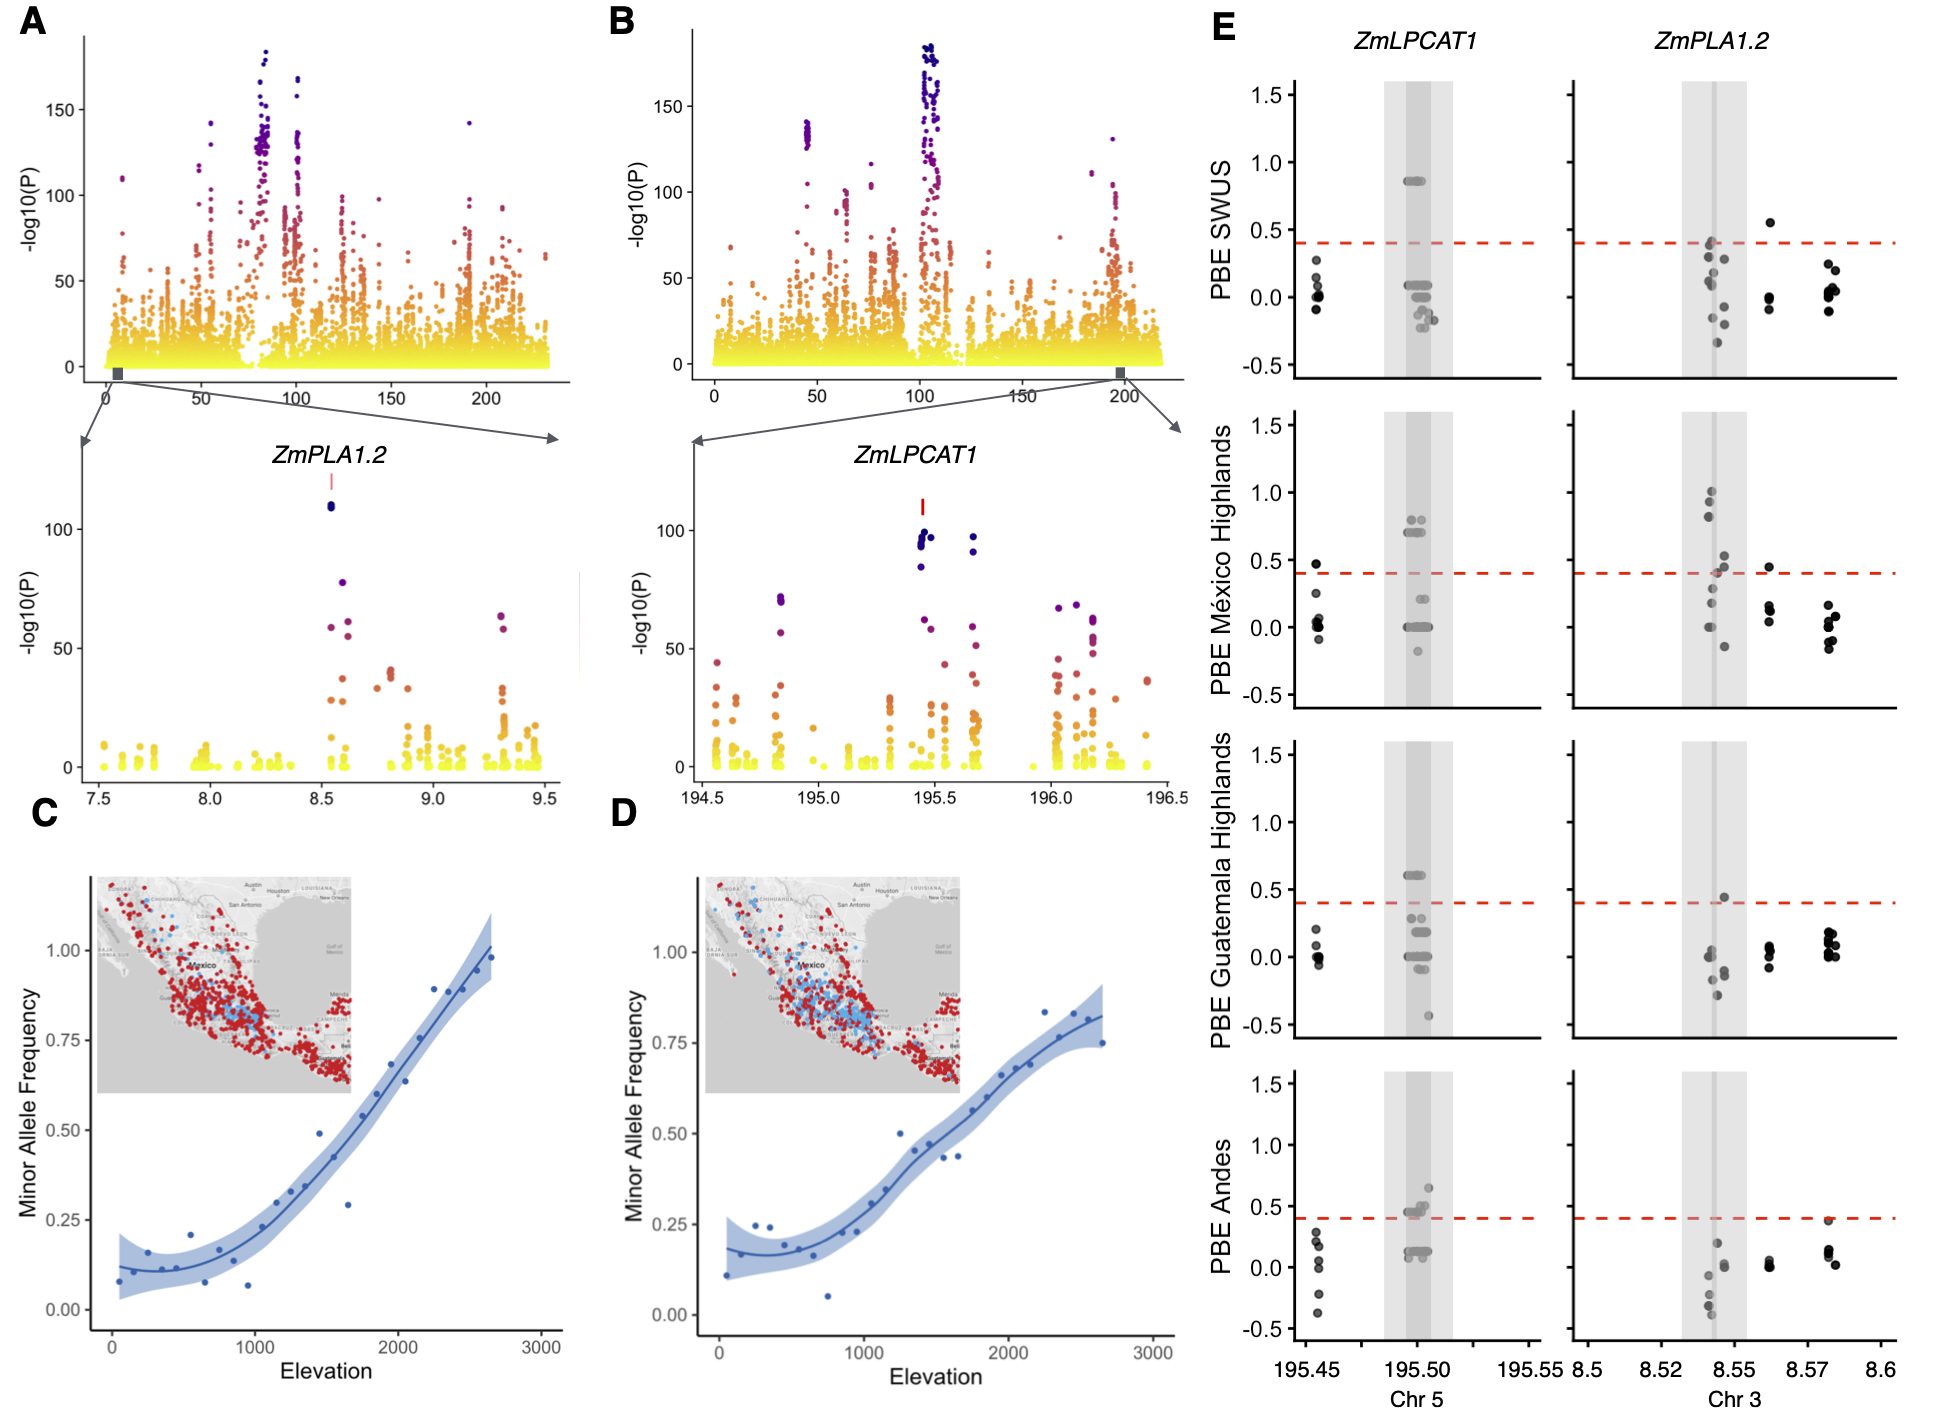
\includegraphics[width=0.4\paperwidth]{Figures/Fig_2.png}
\caption{Manhattan plots of minus log10(P‐values) \textit{Pcadapt} outliers. A) and B) \textit{Pcadapt} PC1 outliers plots of chromosome 3 and 5, respectively. 
Lower panels are zoomed areas of outlier SNPs that colocalize with the physical position of the coding sequences of \textit{ZmPLa1.2} and \textit{ZmLpcat1}. E) and F) show the geographic and elevation dependent frequencies of the highland (blue) and (lowland) alleles of one of the outlier SNPs in the coding sequence of \textit{ZmPLa1.2} and \textit{ZmLpcat1}. 
}
\label{pcadapt}
\end{center}
\end{figure} 

We then used GBS data from 2700 geo-referenced landraces from Mexico generated by the SeeD project \citep{Romero_Navarro2017-cn, Gates2019-we} to run a \textit{pcadapt} analysis that detects genomic regions under selection based on genetic data. We found that the first principal component of \textit{pcadapt} polarizes Mexican landraces based on elevation of origin of the landrace. 
The average -log10(P‐value) of the list of 211 glycerolipid pathways genes was higher than a random sample distribution from the genomic background indicating that glycerolipid pathway genes are under selection on an elevation dependent fashion. Most of the genes that were PBE outliers were also \textit{pcadapt} outliers     

Taken together, these data indicate that both at the gene and the metabolite level, glycerolipid pathways are under selection in highland maize. 
In particular, genes coding for enzymes involved in the synthesis and degradation of phospholipids were convergently selected across different highland populations. 

QTL analysis of phospholipid content in the B73 x Palomero Toluqueño BIL mapping population
Our PBE and lipid analysis of multiple highland and lowland populations across the Americas showed a unique signature of selection for high PC/LPC ratios highland maize from mesoamerica together with selection at the gene level of genes that are involved in determining these metabolic phenotypes. However, these results might be confounded by population structure that is commonly observed in maize landraces (Romero Navarro et al., 2017). We break population structure and further characterize selection and identify loci involved in glycerolipid synthesis in highland maize we developed a bi-parental mapping population using B73, a temperate inbred line, and Palomero Toluqueño (PT) a popcorn, a highland landrace from the Toluca valley in México. We developed 120 BC1S5 backcross Inbred  lines (BILs), using B73 as the recurrent parent (75% B73, 25% PT). This mapping population was grown on the same common garden as the 120 landrace panel and plants were sampled in the same way for glycerolipids analysis. 
Using the sum of lyso-phosphatydilcholines species (LPCs) we found a major QTL peak located at 8.5 Mb of chromosome peak -qLPCs3- (Fig 2A). We also found a major QTL peak -qLPCs3- when we use the sum of phosphatidylcholine species (PCs) (Fig 2B). Effect size plots in this QTL peak show opposite genotypic behaviours. In the case of LPCs (Fig 2C), BILS that are homozygous B73 at the QTL peak, have higher concentrations of LPCs that BILS that are homozygous PT. In the case of PCs (Fig 2D), homozygous B73 BILS at the QTL peak have lower concentrations of PCs than homozygous PT BILS. Based on these results we hypothesized that a locus controlling the PCs/LPCs ratio should be behind  qLPCs3 and qPCs3. We then used the B73 v3 genome assembly and identified 72 genes in the 7.9-10 Mb 99% confidence interval around the QTL peak (Supp file 2). We searched this list of genes for genes that 

\section{Discussion}
\label{sec:discusion}

\section{Acknowledgments}
\label{sec:acknowledgments}

\bibliography{bibliography}

\clearpage

\section*{Supplemental Tables and Figures}

\renewcommand{\thefigure}{S\arabic{figure}}
\linenumbers

\setcounter{figure}{0}

\begin{figure*}[t]
\begin{center}
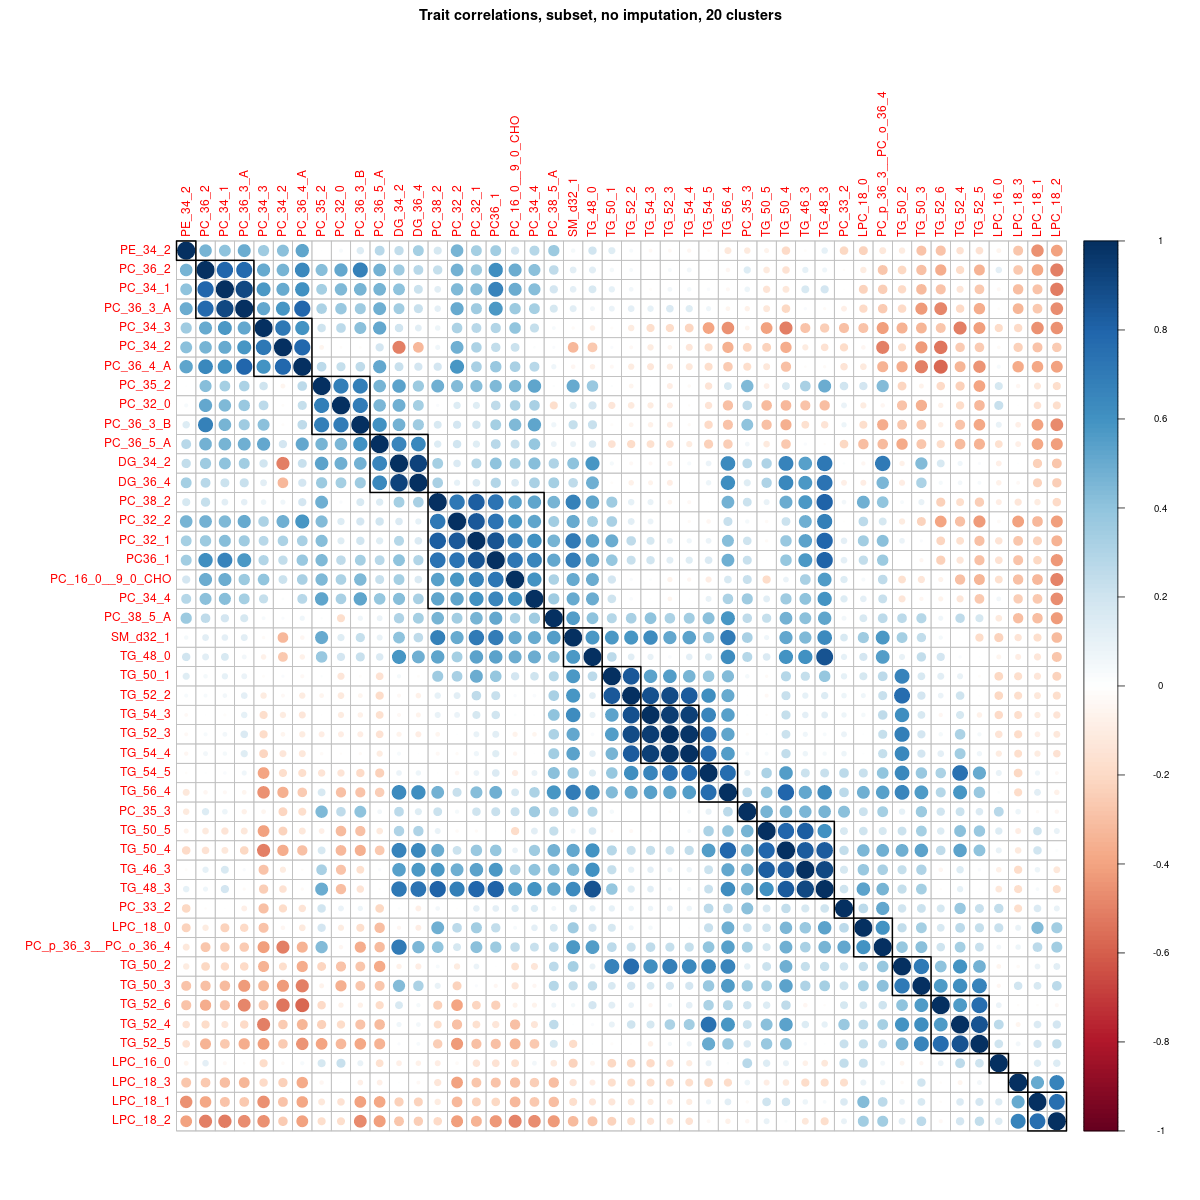
\includegraphics[width=0.4\paperwidth]{Sup_Figures/Sup_Fig_1.png}
\caption{\textit{Pcadapt} analysis of Latin America Landraces. We used GBS data from the Mexican landraces of the SEEDs dataset \citep{Romero_Navarro2017-cn} and run a \textit{pcadat} analysis \citep{Luu2017-ws} that identified (A) elevation as the major driver of genetic differentiation. 
B) Distributions of pcadapt -log10(p values) of PC1 probabilities in a random sample with the average value of pcadapt scores from the glycerolipid PBE outliers in the Mexican highland population shown with a red vertical line . 
}
\label{s-fig1}
\end{center}
\end{figure*} 

\begin{figure*}[t]
\begin{center}
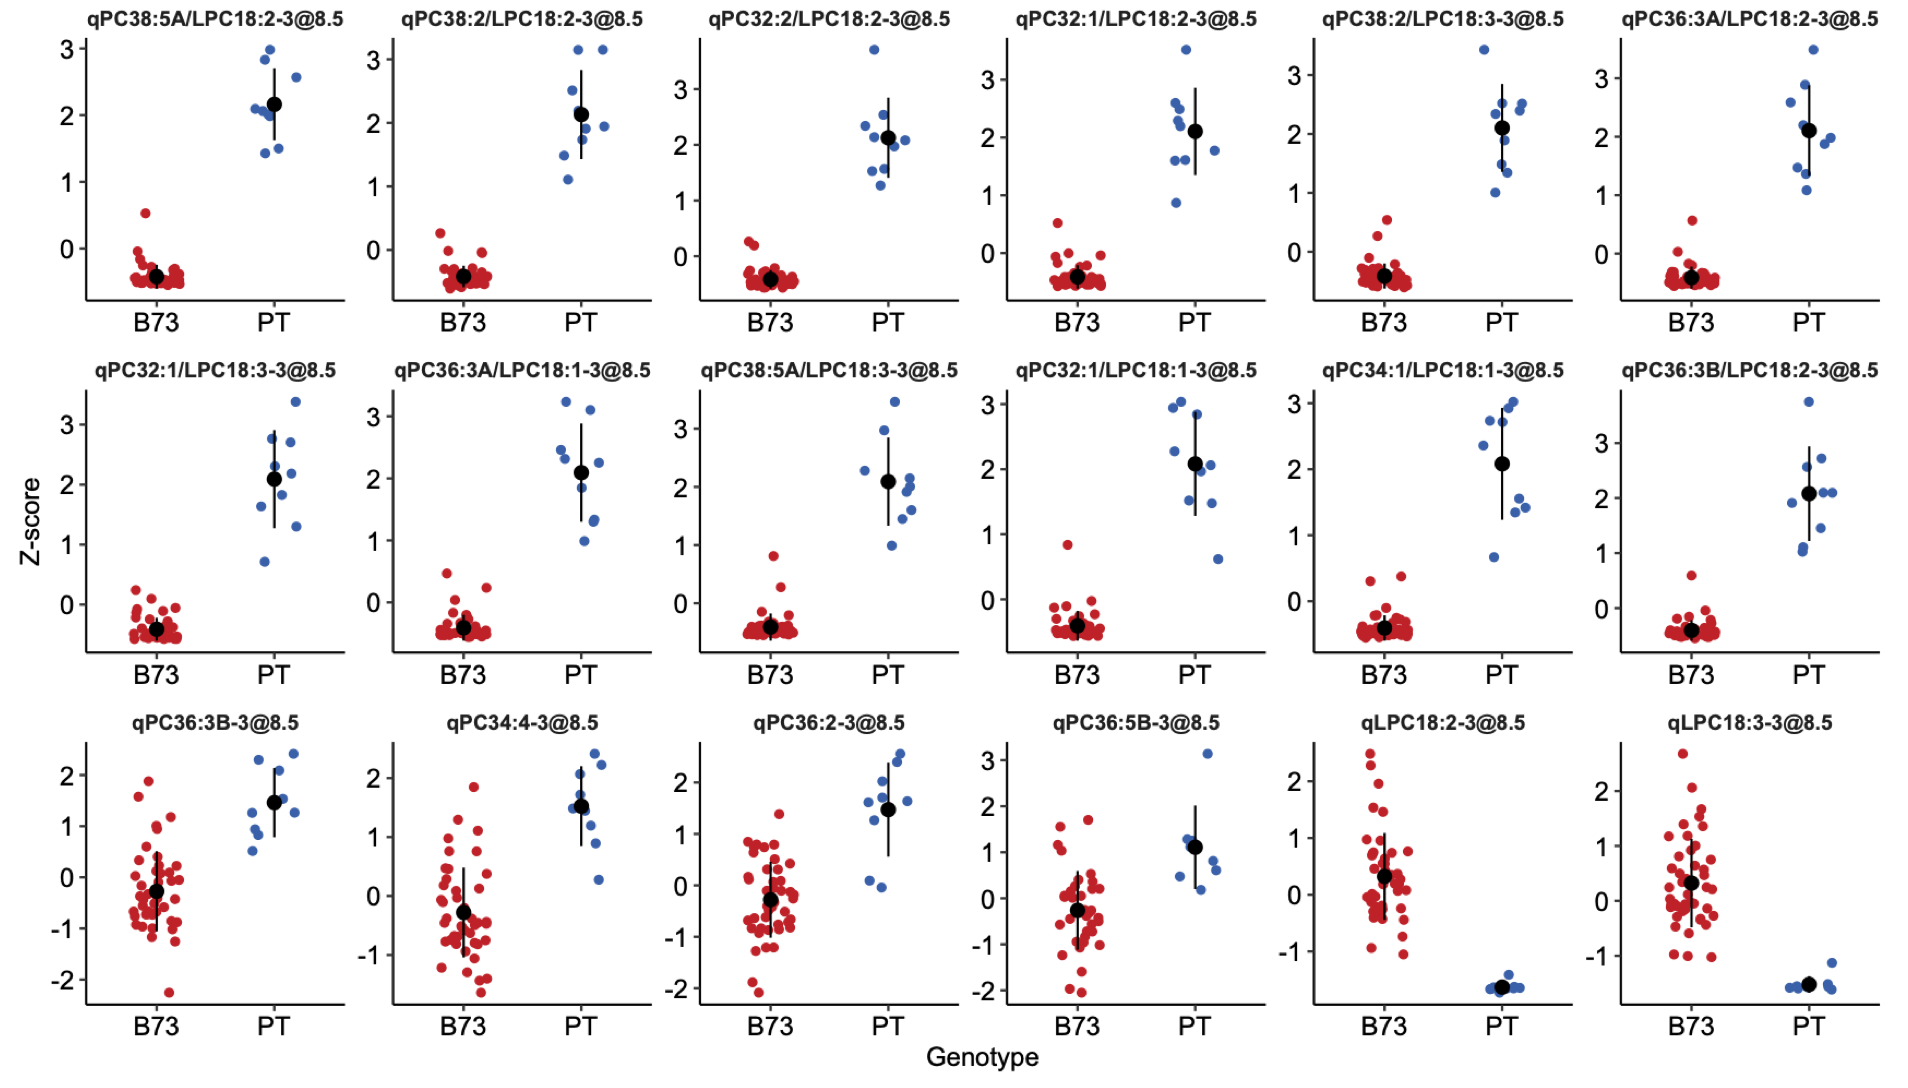
\includegraphics[width=0.4\paperwidth]{Sup_Figures/Sup_Fig_2.png}
\caption{\textit{Qst-Fst} analysis of glycerolipid species analyzed from the 120 Hilo landrace panel. 
}
\label{s-fig1}
\end{center}
\end{figure*} 


\end{document}